\documentclass[a4,center,fleqn]{NAR}
\usepackage{hyperref}
\usepackage{graphicx}
\usepackage{csquotes}
\usepackage{amsmath}
\usepackage{setspace}
\usepackage{float}
\usepackage{caption}
\usepackage{subcaption}
\usepackage[super]{nth}
% Enter dates of publication
\copyrightyear{2017}
\pubdate{18 March 2017}
\pubyear{2017}
\jvolume{37}
\jissue{12}

%\articlesubtype{This is the article type (optional)}

\begin{document}
\title{HiC Contact Map Comaprison Using Graphlet Approach}

\author{%
    Behnam Rasoolian\,$^{1,*}$,
    Debswapna Bhattacharya\,$^{1}$
    \footnote{
    Tel: +1 334 5212814; Email: bzr0014@auburn.edu}}

    \address{%
        $^{1}$ Auburn University
        }
        % Affiliation must include:
        % Department name, institution name, full road and district address,
        % state, Zip or postal code, country

%        \history{%
%            Received January 1, 2009;
%            Revised February 1, 2009;
%            Accepted March 1, 2009}

            \maketitle

\begin{abstract}

In this study, we plan to find dissimilarities between normal cells and cancerous cells,
through investigating HiC contact maps. 
We suspect that there are systematic differences between how chromosomes are structured
between normal cells and cancerous cells.
we 
Ideally, it is desirable to compare 3D structures of 
cell in order to make such comparisons.
However, the main challenge that we face is that 
3D structure of a cell is not readily available. Based on
\cite{adhikari2016chromosome3d}, fluorescence in situ hybridizaiton
(FISH) is used for investigating 3D configuration of chromosomes.
However, this method can only be used locally and cannot map
the whole structure of the chromosomes.
In orther to find dissimilarities in the 3D structure of 
chromosomes, we used HiC dataset.
The HiC method, which was developed by \cite{lieberman2009comprehensive}, captures interactions between 
chromosomal fragments in kilobase resolution. Based on HiC data, an
\textit{interaction frequency (IF) } matrix can be developed between \textit{loci} at a desired resolution.
A cell $IF_{ij}$ in an interaction frequency matrix captures the number of interaction detected
in HiC dataset between locus $i$ and locus $j$ in the genome.
An interaction matrix can be used to develop both inter- and intra-chromosomal interaction matrices.
We believe differences in interaction matrices can be found between normal cells and cancerous ones.
\end{abstract}
\section{Introduction}

Graphlet comparison is a novel method used to compare large networks in order to
find local similarities in them.
Authors of \cite{prvzulj2007biological} provide a new measure of PPI
network comparison
based on 73 constraints. This is used in order to compare two large
networks in order to detect similarities.

\cite{milenkoviae2008uncovering} 
 provide heuristics to compare two nodes based on some feature
(or signature) vectors, which is a 73-dimensional vector
$\mathbf{s}^T
= [s_0, s_2, ..., s_{72}]$ where $s_i$ denotes the number of nodes in
the network that are part of an orbit $i$. \\
\textit{Important Result}: Proteins with similar surroundings perform
similar functions.

In \cite{milenkovic2010cancer}, the same author investigates 
cancer-causing genes to find similarities in their signatures. After
clustering the genes based on \textit{signature similarity} criteria,
some clusters contain a lot of cancerous genes.
They use 4 different clustering methods with varying parameters to cluster
the proteins. They then predict the cancer-relatedness of a protein 
$i$ using
an enrichment criteria $\frac{k}{|C_i|}$ where $C_i$ is the cluster
where protein $i$ belongs and $k$ is the number of cancer-causing
proteins in $C_i$ and $|C_i|$ is the size of $C_i$.


The authors of \cite{di2010fast} generalized the idea of graphlets to 
ordered graphs were the nodes are labeled in ascending order.
As can be viewed, there are a total of 14 orbits for graphlets of size
2 and 3 since the label of graphlets is also included in toplogy.
In the new definition, $d_v^i$ denotes the number of orbit $i$ touches 
node $v$. Each node, is then assigned a vector of length 14 
\footnote{number of orbits in graphlets of size 2 and 3}
$(d_v^1, d_v^2, ..., d_v^{14})$ 
and similarity of two nodes in two contact maps can be compared by
how geometrically close their corresponding vectors are.
\section{Materials and Methods}
\subsubsection{Notations}
In this paper, matrices and vectors are represented as bold
capital and bold small letters respectively.
matrix rows and columns are represented by a \textit{dot}
notation. For example, the $i$th row of matrix $M$ is
denoted by $M_{i.}$ and its $j$th column is represented
by $M_{.j}$.

We denote the set of all contact maps in cell line $T$ with 
$\mathbb{C}^T$. If no particular cell line is addressed, the
subscripts are dropped.
Any arbitrary member of $\mathbb{C}$ is denoted by 
$C_{ij}$, where $i$ and $j$ ($j \ge i$) represent the two chromosomes involved. 
In human cells this set contains a total of 276 contact maps,
23 of which are intra-chromosomal and the rest are inter-chromosomal.
For ease of representations, intra-chromosomal contact maps are
distinguished by a single superscript, so we have $C_{i,i} =
C_i$.

We denote the number of loci in a chromosome $i$ by $N_i$.
The set of all loci involved in contact map $C_{ij}$ is denoted 
by $V_{ij}$.
In intra-chromosomal contact maps, $V_{i,i}$ containts only the 
loci of that particular chromosome ($|V_i| = N_i$), while in 
inter-chromosomal contact maps $V_{ij}$ contains the loci in
the both of chromosomes involved ($|V_{ij}| = N_i + N_j$).

% **************************************************************
% Keep this command to avoid text of first page running into the
% first page footnotes
\enlargethispage{-65.1pt}
% **************************************************************

\subsection{Thresholding contact maps}
In order to be able to extract graphlets, HiC contact maps should be modeled as
unweighted graphs where the nodes represent the loci and an edge between two 
nodes represent a \textit{significant} interaction between the loci.
This can be achieved by thresholding the contact maps. The result
of the thresholding procedure is a binary matrix which also can serve as
an adjacency matrix for an unweighted, undirected graph. The graph can then be
used for orbit extraction.

When thresholding contact maps, it is necessary to make sure
that both global and local features are maintained. We could consider 
thresholding the contact maps by simply setting values above a fixed value to
one and the rest to zero; However, in practice, this method resulted in graphs
that capture the local structure of the contact maps poorly. This is because
intensities follow an exponential distribution with a mean close to zero
with a few very larges values that correspond to interactions along 
or close to the main diagonal of the contact maps.
Thus, picking relatively large numbers would result in ignoring interactions
that are far from the main diagonal while picking small values will lead to
capturing too many (insignificant) interactions.

In order to threshold the matrix so that both global and local patterns are
captured, we borrowed the concept of \textit{adaptive thresholding} from image 
processing context. In this method, in order to be set, a pixel should have
an intensity larger than the average of non-zero intensities in its
\textit{neighborhood}. The neighborhood is defined by a sliding kernel 
that passes through the contact map with the pixel at its middle at 
each step. Figure \ref{local_thresholded_chr1_chr1} demonstrates result of 
this thresholding approach for intra-chromosomal contact maps of chromosome 1.
Refer to supplementary material for all 23 interchromosomal thresholding
results.
\begin{figure}[t]
    \centering
    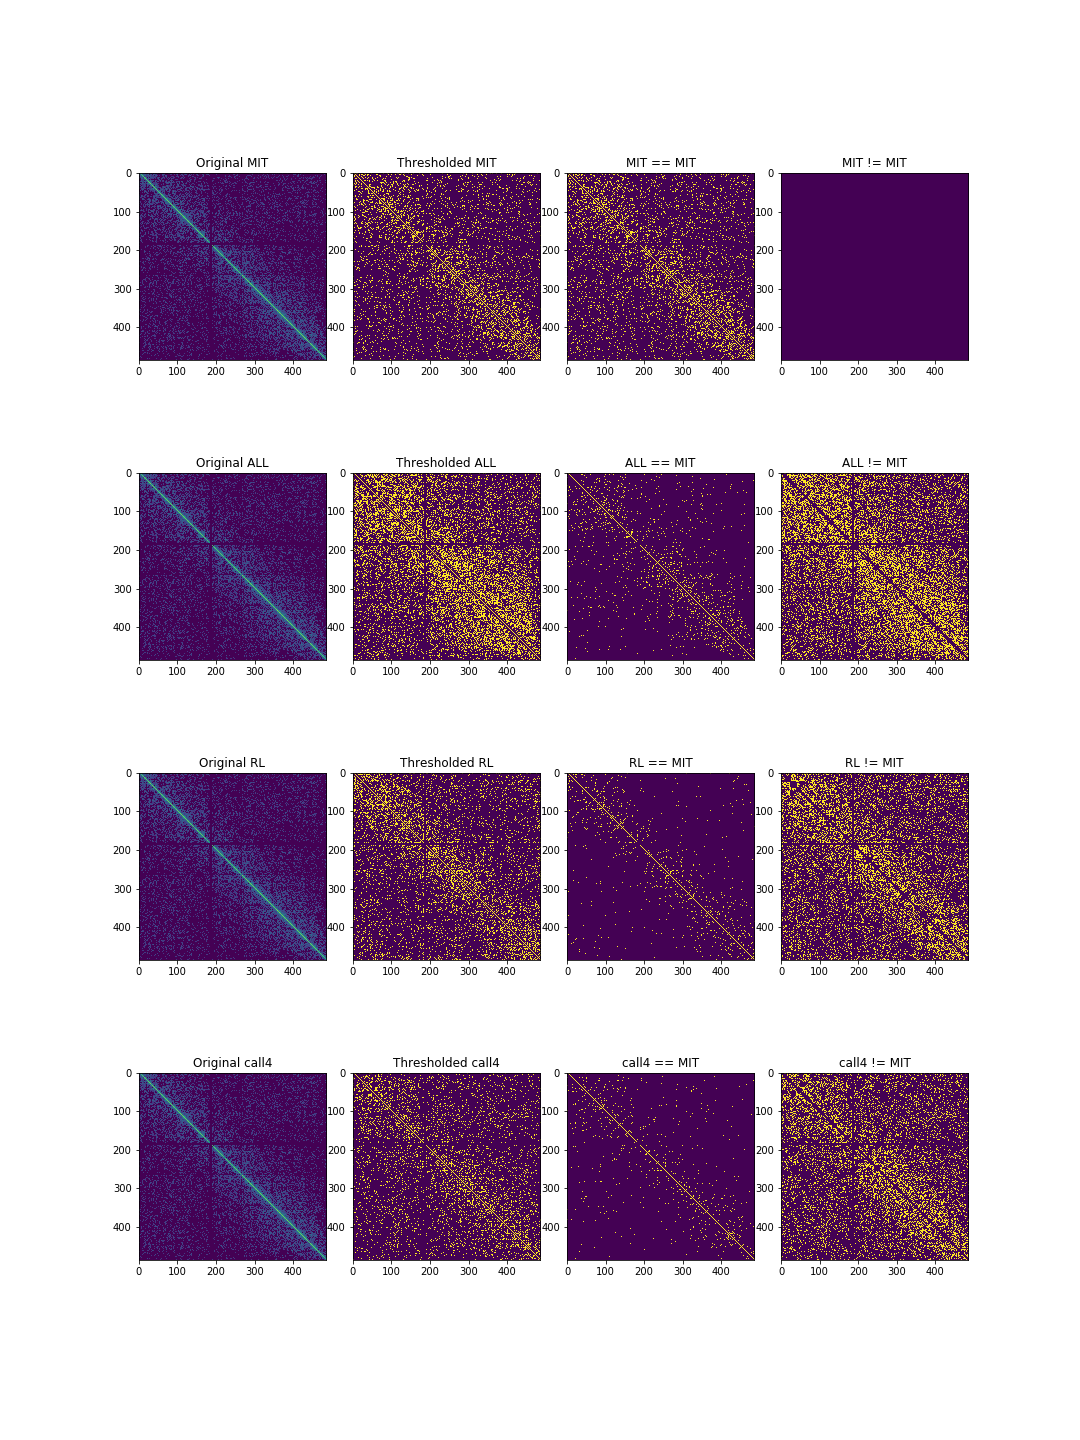
\includegraphics[width=.5\textwidth]{figures/local_thresholded_chr1_chr1.png}
    \caption{Result of thresholding interchromosomal contact map of chromosome 1
    using a kernels of size $5 \times 5$ for all cell lines. 
    The first row shows the thresholded
    maps. Second and third rows demonstrate pair-wise similarities and 
    differences between contact maps respectively.}
    \label{local_thresholded_chr1_chr1}
\end{figure}

\subsection{Orbit Extraction}
Once the thresholded contact maps are obtained, graphlets and orbits can be 
extracted. We used the \texttt{orca} package in \texttt{R} programming 
language to extract the graphlets. As a result of graphlet extraction, 
For each loci in each contact map, a \textit{signature vector} of size
73 is created. Thus for each cell line, we would have 276 
\textit{signature matrices} of
size $|V^{ij}|\times 73$, where $V^{ij}$ is the number of loci
involved in contact map between chromosomes $i$ and $j$. Figure
\ref{fig:graphlet_extraction} illustrates the process and results
of signature matrix extraction schematically.
\begin{figure}
    \centering
    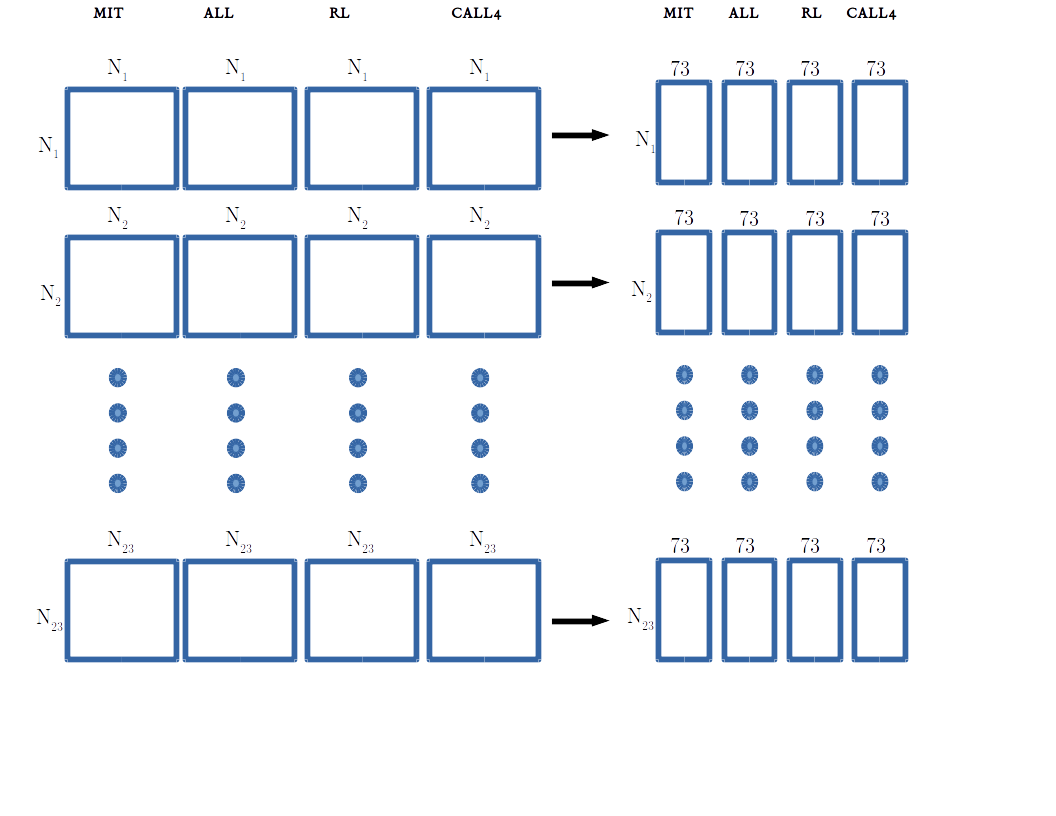
\includegraphics[width=.5\textwidth]{figures/graphlet_extraction.png}
    \caption{Graphlet extraction for the four cell lines. For each
    loci in each contact map between chromosomes $i$ and $j$, 
    the signature vectors of length 73 are extracted, resulting 
    in a \textit{signature matrix} of size $|V^{ij}| \times 73$,
    where $V^{ij}$ 
    is the number of loci involved.}
    \label{fig:graphlet_extraction}
\end{figure}

For a particular
$\mathbf{C}_{ij}$, we denote $\mathbf{S}_{ij}$ as its \textit{signature 
matrix}. Each cell $S_{ijlo}$ in $\mathbf{S}_{ij}$ captures how many
times loci $l$ in $\mathbf{C}_{ij}$ occured as part of orbit $o$.


\begin{figure}
    \centering
    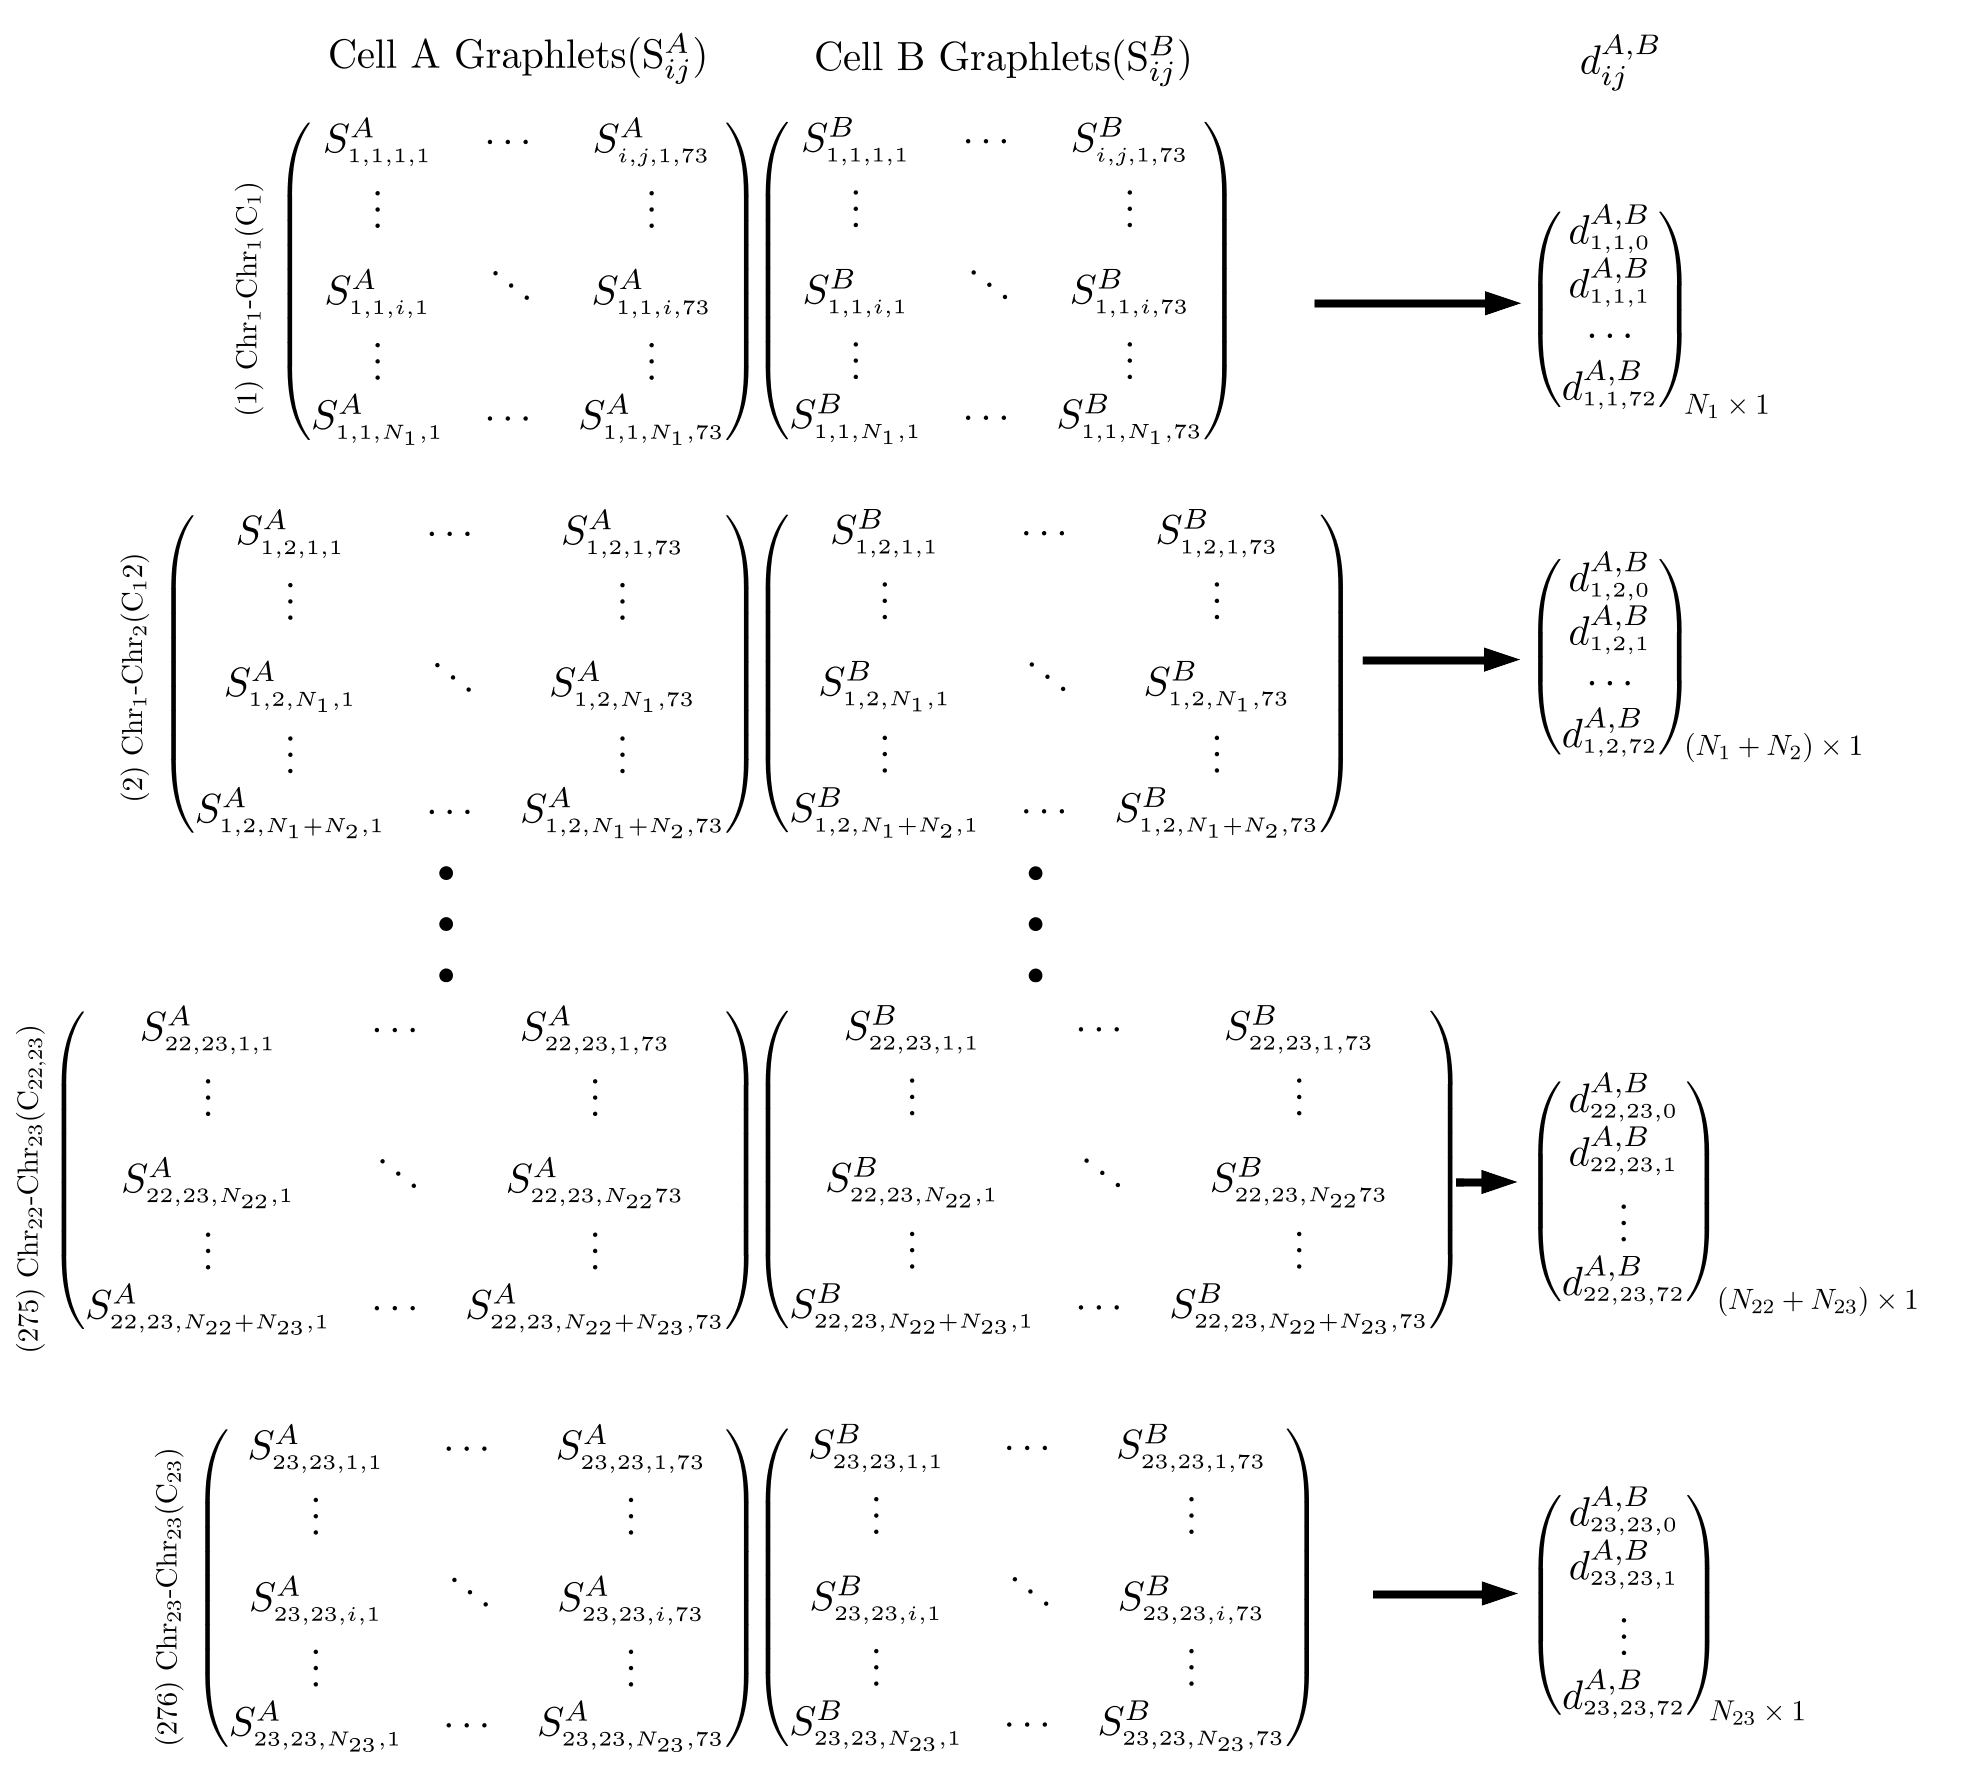
\includegraphics[width=.5\textwidth]{figures/graphlet_distance_schema.png}
    \caption{Calculating pair-wise loci distances. For each loci (row) 
    in each
    contact map in MIT cell line, its distance is calculated based on
    equation \ref{eq:distance_total} with the corresponding loci in
    leukemic cells. The result of this process is a 
    \textit{signature distance vector} of size
    $|V^{ij}| = N_i+N_j$ for each contact map.
    }
    \label{graphlet_distance_schema}
\end{figure}
\begin{figure}
    \centering
    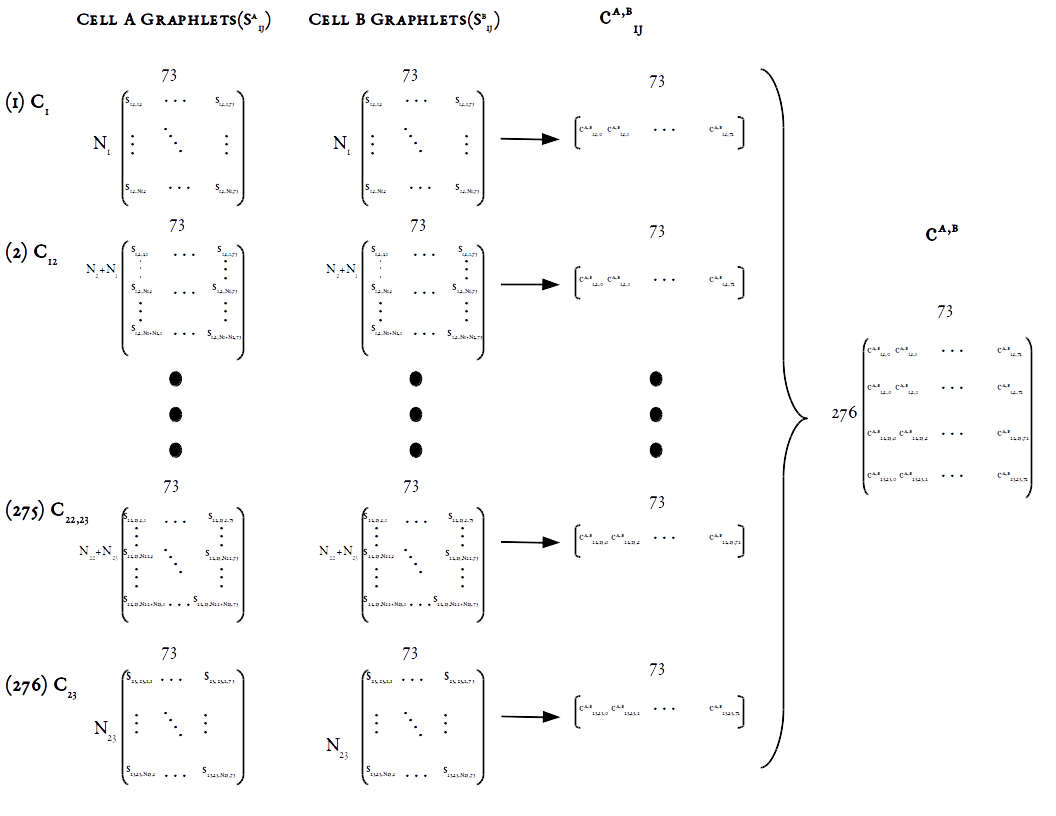
\includegraphics[width=.5\textwidth]{figures/graphlet_correlation_schema.png}
    \caption{Calulating pair-wise orbit correlations. For each orbit (column)
    in each contact map in MIT cell line, its correlation with the
    same orbit in the same contact map 
    in leukemic cells is calculated. The result of
    this process is a \textit{signature correlation} vector of size
    73 which captures how similar frequencies of two orbits are.
    In order to test our second hypothesis, we calculated averages
    across contact maps (along the vertical red arrow) to test 
    hypothesis \ref{eq:h2a}
    and across orbits
    (along the horizontal red arrows) to test hypothesis \ref{eq:h2b}.}
    \label{graphlet_correlation_schema}
\end{figure}

%We divided the task of graphlet comparison into two parts: first we compare
%graphlets from each contact map in normal cell lines (MIT) with the 
%same contact maps in the other three Leukemic cells. Second we compare 
%contact maps in a similar way but this time only between leukemic cells.
%In the former case, the null hypothesis is that there is no difference
%between contact maps of normal cells and leukemic cells and in the latter
%case, the null hypotheis is that there is no difference between 
%different leukemic cells.

We consider two measures of \textit{difference} when comparing contact
map graphlets across cell lines. 
The first measure is \textit{signature distance vectors} between
each contact map of two cell lines. 
For a pair of cells A and B, let 
$\mathbf{S}^A_{ij}$  and $\mathbf{S}^B_{ij}$ be their
signature matrices. The \textit{signature distance} of
contact map $\mathbf{C}_{i,j}$ between A and B is denoted
by $\mathbf{d}^{\scriptscriptstyle A,B}_{ij}$. $\mathbf{d}^{\scriptscriptstyle A,B}_{ij}$ 
is a vector of size $|V_{i,j}|$
and its elements $d^{\scriptscriptstyle A,B}_{i,j,l}$ are
calculated using the following formula from \cite{prvzulj2007biological}:

\begin{equation}
    d^{\scriptscriptstyle A,B}_{i,j,l} = 
    \frac{1}{73}\sqrt{\sum_{o=0}^{72}{t_{lo}^2}}
    \label{eq:distance_total}
\end{equation}

where elements of $t_{i,j,l,o}$ is the
distance between each
loci (row) $l$ in $\mathbf{S}^A$ and the the same loci in 
$\mathbf{S}^B$ for
orbit $o$ as is calculated as below:

\begin{equation}
    t_{lo} = w_o \times 
    \frac{log(S_{ijlo}^A+1) - log(S_{ijlo}^B+1)}
    {log(max(S_{ijlo}^A, S_{ijlo}^B) + 2)}
    \label{eq:distance_single}
\end{equation}


This process is illustrated in Figure \ref{graphlet_distance_schema}.
Using this distance measure, we can quantify how two loci are close to
each other in terms of local neighborhood between the two contact maps.

The second measure of comparison that we use captures how 
similar two orbits are in terms of their count 
frequencies across loci between two contact maps. 
Each column in $S_{ij}$ can provide information
regarding the \textit{frequency distribution} of orbits throughout
the contact map $C_{ij}$. 
We can find how similar these distributions are to each other using
correlation measures.
These correlations are denoted by $\mathbf{m}^{\scriptscriptstyle A,B}_{i,j}$ and
can be calculate using
any plausible correlation measure. 
In this study, for each contact map,  we calculated
similarity between orbit distributions using Pearson's r 
correlation, which is computationally efficient.
However, pearson's r might not be able to capture
non-functional relationships between distributions. As a result, we
also used Maximal Information Coefficient (MIC) 
\cite{reshef2011detecting} in order to compare
correlations. MIC calculates mutual information (MI) between two
distributions, but utilizes dynamic programming in order adjust
bin sizes and numbers in order to achieve highest MI.
MIC values between two variables fall between 0 and 1,
with 0 meaning the two variables are completely independent
and 1 meaning one is dependant on the other.
We used both Pearson's r and MI in order to compare orbit
frequencies. Although results from both approaches were more
or less consistent, MIC showed higher robustness than Pearson's 
r method.

If MIC is used as correlation measure, each element of 
 $\mathbf{c}$ is calculated as below:
\begin{equation}
    m^{\scriptscriptstyle A,B}_{ijo} = MIC(\mathbf{S}^A_{ij.o}, \mathbf{S}^B_{ij.o})
    \label{eq:mic}
\end{equation}
Alternatively, if we use Pearson criterion we would have:
\begin{equation}
    m^{\scriptscriptstyle A,B}_{ijo} = Pearson(\mathbf{S}^A_{ij.o}, \mathbf{S}^B_{ij.o})
    \label{eq:pearson}
\end{equation}

\section{results}

Result of pair-wise contact map graphlet distances can is
illustrated in Figure \ref{fig:orbit-distances}.
Each point on the graph is the
average of the graphlet distance vector 
($\bar{\mathbf{d}}^{\scriptscriptstyle A,B}_{i,j}$)
of the two cell lines specified in the legend.
 A one sided paired t-test
was conducted . The resulting p-values showed highly 
significant differeces from zero for all pairs of
cells. Detailed results of t-tests for each
contact map can be fount in supplementary materials.
For each contact map, each pair of cells are
order based on whether they are statistially
larger that the other or not. For example
for contact map $C_{i,j}$, the results 
of t-test is as follows:
\vspace{.2cm}\\
\small{
zero  $<$  call4-mit  $<$     all-rl  $<$     mit-rl  $<$   call4-rl  $<$    all-mit  $=$  all-call4
}
\vspace{.2cm}\\
which means that $\mathbf{d}^{\scriptscriptstyle CALL4, MIT}_{1,1}$ is statistically larger than 0,
but less than $\mathbf{d}^{\scriptscriptstyle ALL, RL}_{1,1}$ 
and so forth. We can also conclude that $\mathbf{d}^{\scriptscriptstyle ALL, CALL4}_{1,1}$ is not
statistically different from $\mathbf{d}^{\scriptscriptstyle ALL, MIT}_{1,1}$
between graphlets extracted from all contact maps. 
Refer to supplementary
material for results of all hypotheis tests.

\begin{figure*}[t]
    \centering
    \begin{subfigure}[b]{\textwidth}
        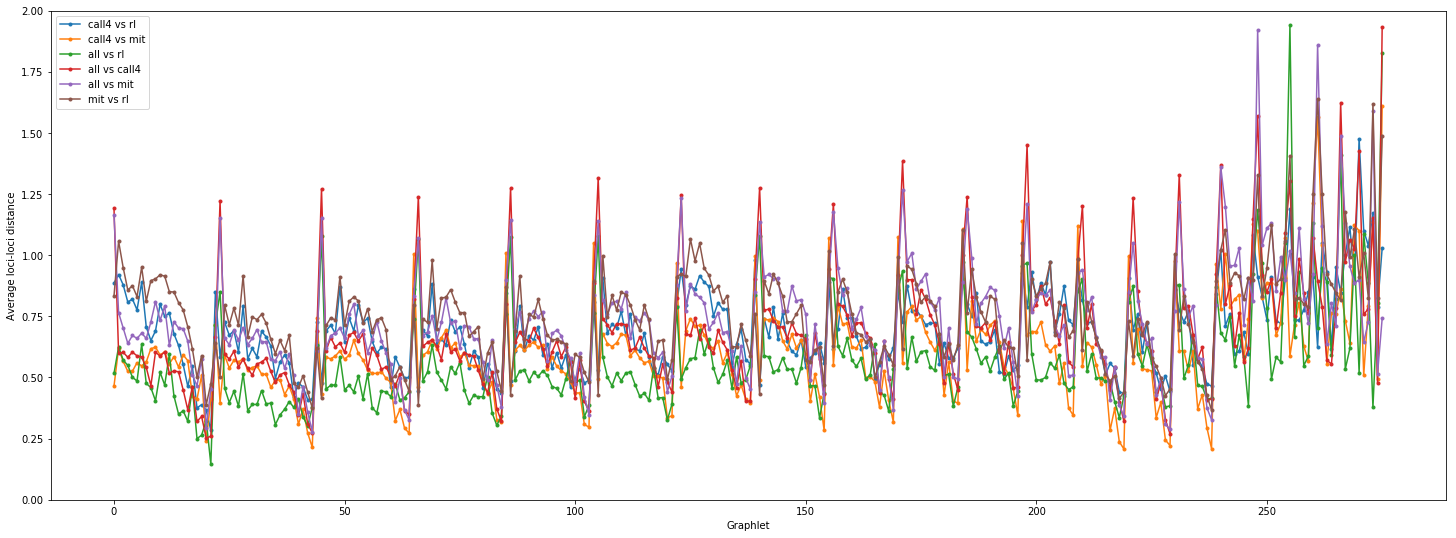
\includegraphics[width=\textwidth]{figures/orbit-distances_all.png}
        \caption{}
        \label{fig:orbit-distances_all}
    \end{subfigure}

    \begin{subfigure}[b]{\textwidth}
        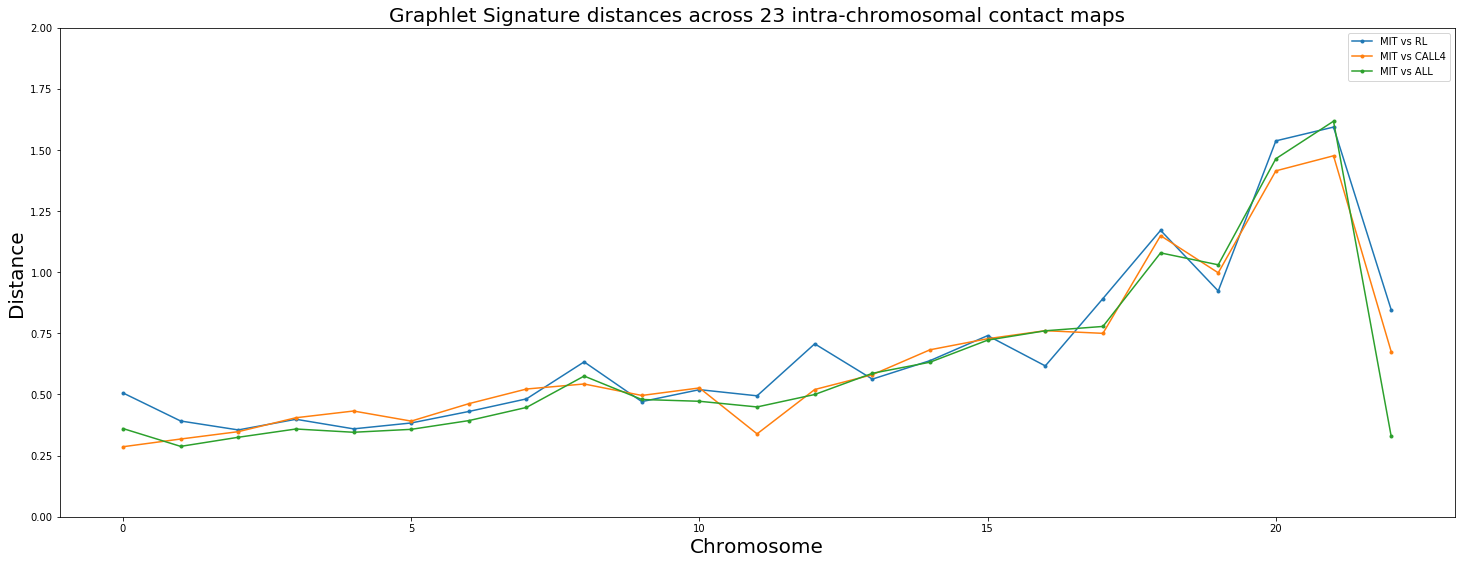
\includegraphics[width=\textwidth]{figures/orbit-distances_intra.png}
        \caption{}
        \label{fig:orbit-distances_intra}
    \end{subfigure}
    \begin{subfigure}[b]{\textwidth}
        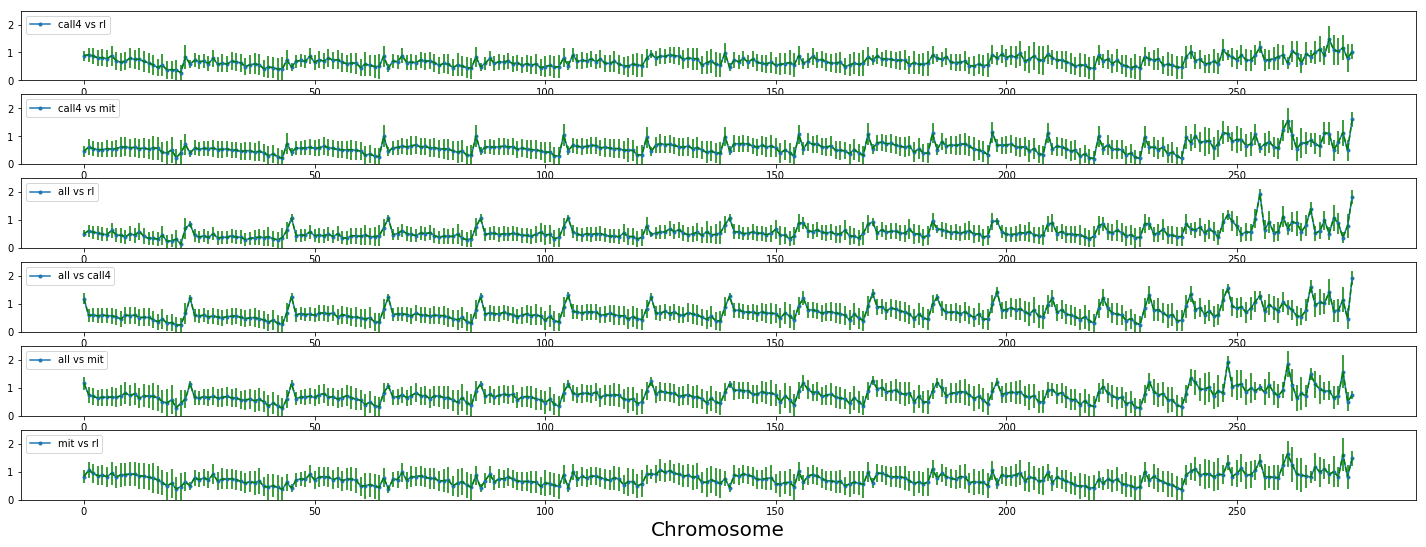
\includegraphics[width=\textwidth]{figures/orbit-distances_intra_separate.png}
        \caption{}
        \label{fig:orbit-distances_intra_separate}
    \end{subfigure}
    \caption{   Pair-wise graphlet signature difference for
                (\textbf{a}) all 276 contact maps
                ($\bar{\mathbf{d}}^{\scriptscriptstyle A,B}_{i,j} \quad
                \forall i,j \in \{1 ... 23\} \quad \& \quad j \ge i$).
                (\textbf{b}) only the 23 intra-chromosomal contact maps
                ($\bar{\mathbf{d}}^{\scriptscriptstyle A,B}_{i,i}$).
                (\textbf{c}) all 276 contact maps as well as corresponding
                standard errors.
                Each point on a graph is the result of averaging all
                the distances acroos all loci of that contact map.
                As can be viewd, although inter-chromosomal graphlets 
                do not show significant differences, RL's inter-chromosomal
                graphlets seem to be closer to MIT's. Also in some contact
                maps ALL graphlets show greater distance from MIT graphlets
                than the other two cell lines.
             }
    \label{fig:orbit-distances}
\end{figure*}

We caclulated pair-wise MIC for each orbit in each of the 276
contact maps from MIT data and ALL, RL and CALL4 data separately. 
Figure \ref{fig:contact_maps_correlations}
shows average orbit correlations across all contact maps, while
figure \ref{fig:orbits_correlations} 
demonstrates average correlations across all 72 orbits within each  contact map.
It is worth mentioning that \textit{interchromosomal} thresholded contact maps 
represent
a bipartide graph with the loci from each chromosome on one side. Due to this
bipartide nature of the graphs in inter-chromosomal maps,
count of certain orbits is always 0, resulting in
a correlation values of 0 for them as well.
We ignored these values  when we calculated averages across orbits 
in figure \ref{fig:contact_maps_correlations_all} since they
would result in a bias towards zero in averages. You can see the bias in 
figure \ref{fig:orbits_correlations_all} where average correlations of orbits
$\mathbb{Q} = \{3, 9, 10{\text -}14, 20{\text -}34, 39{\text -}48, 51{\text -}72\}$ 
are close to zero. In fact all correlations
corresponding to these orbits are 0 except for the ones between the same 
chromosomes which are illustrated in Figure 
\ref{fig:orbits_correlations_intra}.

\begin{figure*}[t]
    \centering
    \begin{subfigure}[b]{\textwidth}
        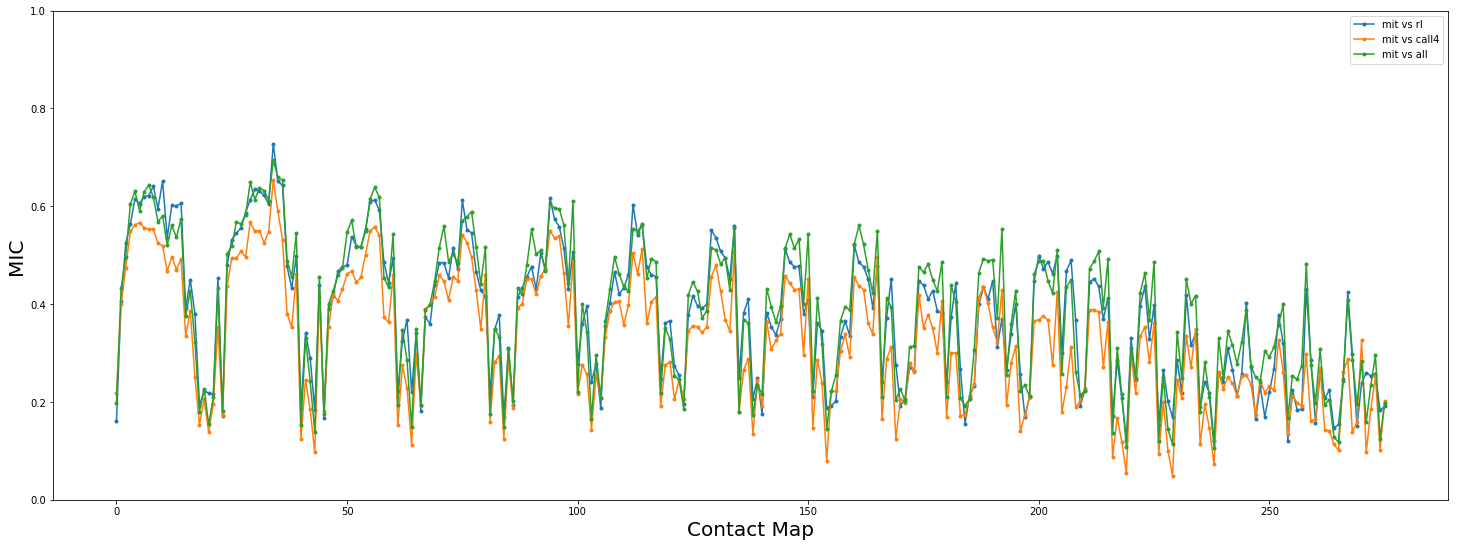
\includegraphics[width=\textwidth]{figures/contact_maps_correlations_all.png}
        \caption{}
        \label{fig:contact_maps_correlations_all}
    \end{subfigure}
    \begin{subfigure}[b]{\textwidth}
        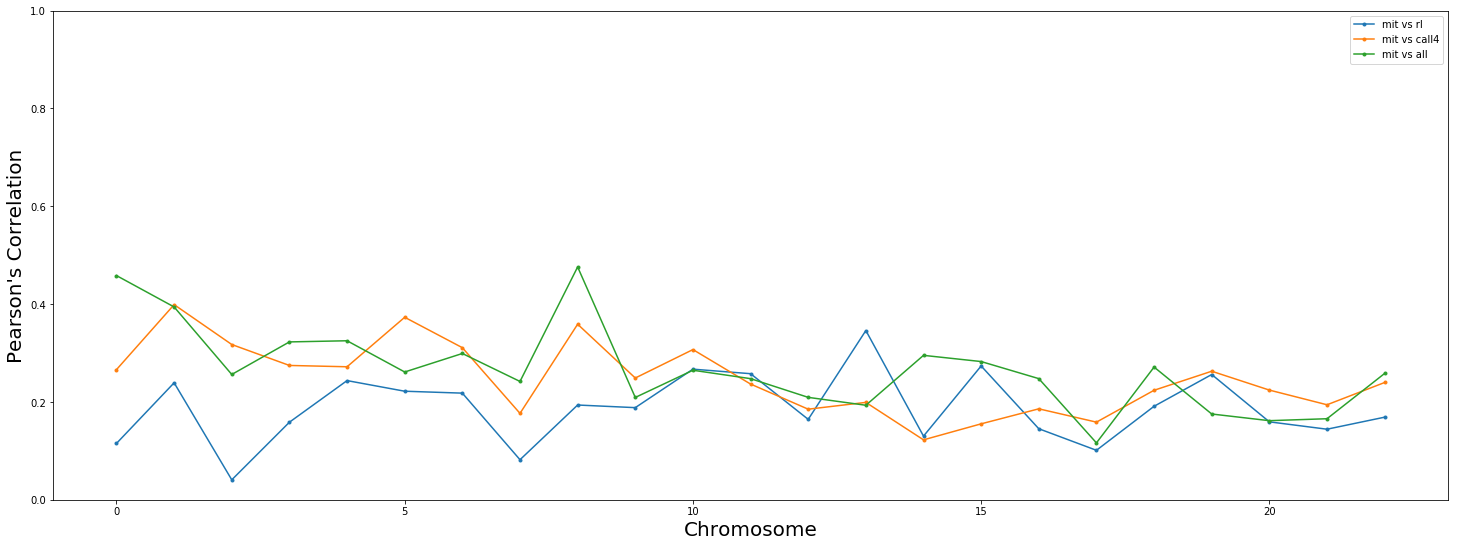
\includegraphics[width=\textwidth]{figures/contact_maps_correlations_intra.png}
        \caption{}
        \label{fig:contact_maps_correlations_intra}
    \end{subfigure}
    \caption{pair-wise average contact map orbit correlations
             (a) for all contact maps($\bar{\mathbf{m}}^{\scriptscriptstyle \scriptscriptstyle A,B}_{i,j} 
            \quad \forall i,j \in \{1 ... 23\} \quad \& \quad j \ge i$,
            average along the red \textit{vertical} arrow in figure 
            \ref{graphlet_correlation_schema})
             (b) only for intra-chromosomal contact maps
            ($\bar{\mathbf{m}}^{\scriptscriptstyle \scriptscriptstyle A,B}_{i,i} 
            \quad \forall i \in \{1 ... 23\} $)
             These values are calculated by averaging over 
             pairwise correlations of all orbits in a 
             contact map.
             }
    \label{fig:contact_maps_correlations}
\end{figure*}

\begin{figure*}[t]
    \centering
    \begin{subfigure}[b]{\textwidth}
        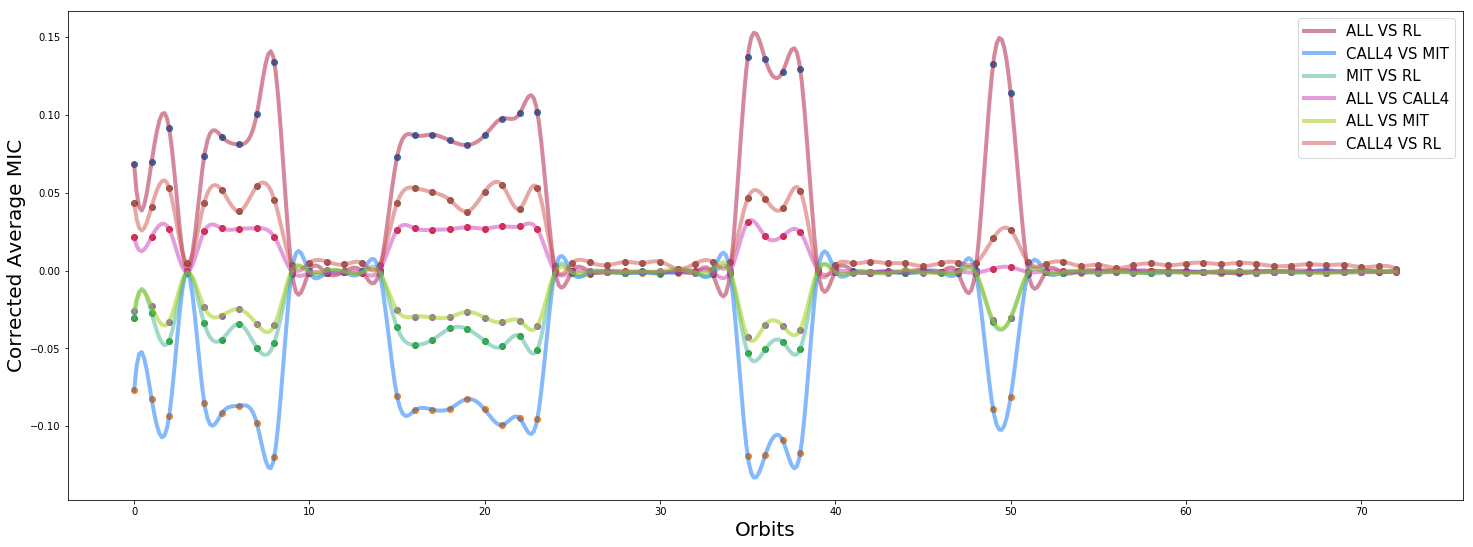
\includegraphics[width=\textwidth, height=.2\paperheight]{figures/orbits_correlations_all.png}
        \caption{}
        \label{fig:orbits_correlations_all}
    \end{subfigure}
    \begin{subfigure}[b]{\textwidth}
        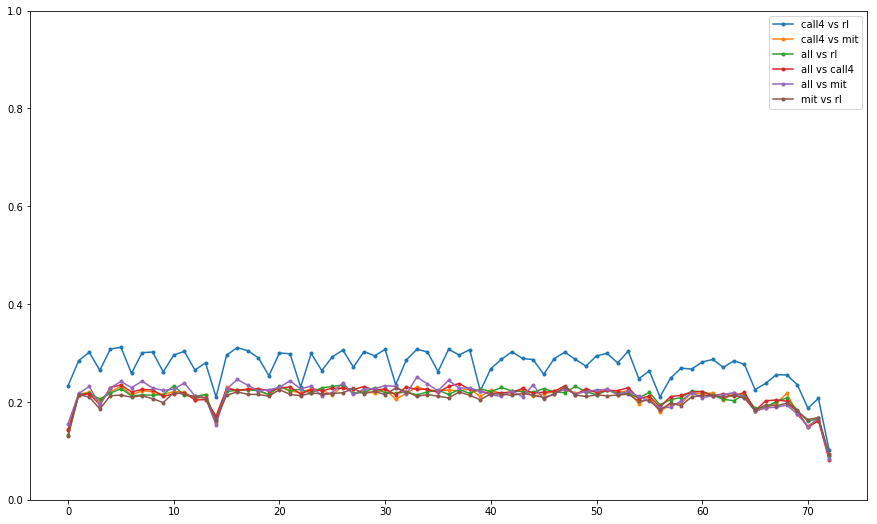
\includegraphics[width=\textwidth, height=.2\paperheight]{figures/orbits_correlations_intra.png}
        \caption{}
        \label{fig:orbits_correlations_intra}
    \end{subfigure}
    \caption{pair-wise average orbit correlations.
             In figure \ref{fig:orbits_correlations_all}, each point
             in the graph is the result of averaging pair-wise
             orbit correlations over all contact maps
             ($\frac{1}{276}\sum_{i=0}^{23}\sum_{j=i}^{23}{
             m^{\scriptscriptstyle \scriptscriptstyle A,B}_{i,j, o}} \quad 
             \forall o \in \{0, 1, ..., 72\}$,
             average along the red \textit{horizontal} arrows in figure 
             \ref{graphlet_correlation_schema}), while
             each point in figure \ref{fig:orbits_correlations_intra}
             are averaged only over intra-chromosomal contact maps
             ($\frac{1}{23}\sum_{i=0}^{23}{
             m^{\scriptscriptstyle \scriptscriptstyle A,B}_{i,i, o}} \quad 
         \forall o \in \{0, 1, ..., 72\}$).
             Counts for certain orbits are always zero in inter-chromosomal
             maps, leading to average value close to zero in 
             \ref{fig:orbits_correlations_all}.
             }
    \label{fig:orbits_correlations}
\end{figure*}
We have conducted one-sided
t-test in order to test whether the average correlations across
contact maps is equal to 1  and whether the average 
correlations across orbits is equal to 1. The results
for both test showed that all values are significantly less than 1.
Please refer to supplementary material for result of the t-tests.

\section{discussion}
\newpage
\section{Resources}
\textbf{Hi-C Datasets:}
\begin{enumerate}
    \item \href{https://github.com/rasoolianbehnam/watson}{Code base for this article}
    \item \href{http://sysbio.rnet.missouri.edu/T0510/tmp_download/link_to_download_genome_data/}
        {Datasets including cancerous cells}
    \item \href{https://bcm.app.box.com/v/aidenlab/folder/11234760671}{Original Datasets}
\end{enumerate}


\bibliography{lit}
\bibliographystyle{unsrt}
\end{document}
